\documentclass[tikz,border=9pt]{standalone}
\usepackage{amsmath,amssymb}
\usetikzlibrary{arrows.meta,positioning,calc}
\begin{document}
\begin{tikzpicture}[font=\small,arr/.style={-{Stealth},thick},box/.style={draw=blue!55!black,rounded corners,fill=blue!4,align=center,text width=2.9cm,minimum height=1.05cm}]

\node at (0,0){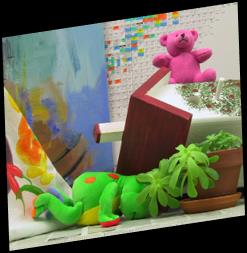
\includegraphics[height=4cm]{book/images/lecture04/sources/plant-left.jpg}};
\node at (6,0){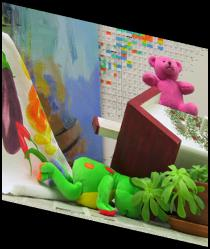
\includegraphics[height=4cm]{book/images/lecture04/sources/plant-right.jpg}};
\node at (0,2.5){Reference image};\node at (6,2.5){Matching image};
\node[align=center] at (3,-2.8){Find the same visible surface, not just the same color.\\Depth changes its location between views.};

\end{tikzpicture}
\end{document}
